%%% The first section of your paper. 

\section{Introduction}

CAD applications are widely popular in product design. They aid the design process in presenting easy-to-use ways of defining shapes, attributes, relationships etc. Shapes modeled in CAD can then be used in various downstream applications like drafting, analysis, manufacturing etc. Many commercial CAD applications provide {\em Design-by-Features} approach. Features, not only carry shape information (geometry, topology) but also embed meta-information based on the application's need. Features also reflect terminologies used in the application, thus making them intuitive to use. But this has given rise to various feature-schema not only in different CAD applications but also in various environments present within the same CAD application. Shape that a feature represents could be similar but its feature-nomenclature, usage, could be different in different environments-applications. Features like {\em Box}, {\em Pad}, {\em Protrusion}, {\em Extrude}, appear different in nomenclature, but all could be representing the same shape. This diversity of vocabulary creates problems in learning new CAD systems, interoperability between different CAD applications, and also in development of functionality for downstream applications. This is evident in relatively lesser usage of features in the downstream applications, especially, CAE.  Instead of plethora of feature nomenclatures, a neutral-standardized internal representation can be devised. Functionality developed on top of such representation will have advantage of applicability over variety of feature representations present in different CAD applications.

This paper presents an idea of formalizing form features in terms of  Spatial Grammars notations and  and demonstrates its use in developing algorithms on top of it, for downstream applications, like {\em Midsurface} for CAE. 

\section{Related Work}

	Following subsections explore salient work done so far in the areas relevant to the topic, like,  Spatial Grammars , Form Feature Representation and Midsurface Representation.

\subsection{Spatial Grammars}

 Spatial Grammars is a general term which encompasses shape definition Grammars, like Graph Grammars, Shape Grammars, Set Grammars, etc. Aim of  Spatial Grammars is to bring formalism through terse but expressive definitions, validations and generation of new evolutionary shapes. Although primarily used for generative designs in architecture, Hoisl et al.\cite{Hoisl2012}  proposed a  Spatial Grammars based system for implementation in CAD, for generative solutions. CAD Grammars proposed by Deak et al.\cite{Deak2006} combined Shape and Graph Grammars to be more useful in Design, Modeling and Manufacturing. In general there has been limited success to the usage of Spatial Grammars in CAD-CAE due to its complexity of formulation and non-intuitive user interfaces.

\subsection{Form Feature Representation}

A generally accepted definition of feature is that  it represents shape as well as functionality significant to particular product life-cycle phase. Features through use of taxonomy, semantics and ontology  bring formalized knowledge representation which can be leveraged to address problems such as interoperability between CAD system and developing downstream applications such as CAE, CAM etc \cite{BidarraBronsvoort2000}.

%A generally accepted definition of feature is that  it represents shape as well as functionality significant to a particular product life-cycle phase. Features embed application specific high level knowledge and manifest differently as per the context . Features through use of taxonomy, semantics and ontology  bring formalized knowledge representation which can be leveraged to address problems such as interoperability between CAD system and developing downstream applications such as CAE, CAM etc.

Use of  Spatial Grammars notations to represent scheme of generalized {\em form features} is relatively new and is not widely utilized in the commercial CAD applications. This paper formalizes an approach to  such representation and later uses it to develop {\em Midsurface} which is an important idealization method in CAE.


\subsection{Midsuface Representation}

Midsurface is an abstraction of thin-walled portions of solid into a set of connected surfaces that lie midway and carry thickness information needed to define 2D shell elements  (Figure \ref{figure_Midsurf}). There are various techniques to extract Midsurface mentioned in academic world and available in commercial CAD-CAE applications. Predominant among those techniques are, Medial Axis Transform (MAT) and Midsurface Abstraction (MA) method. 

	\begin{figure}[h]
	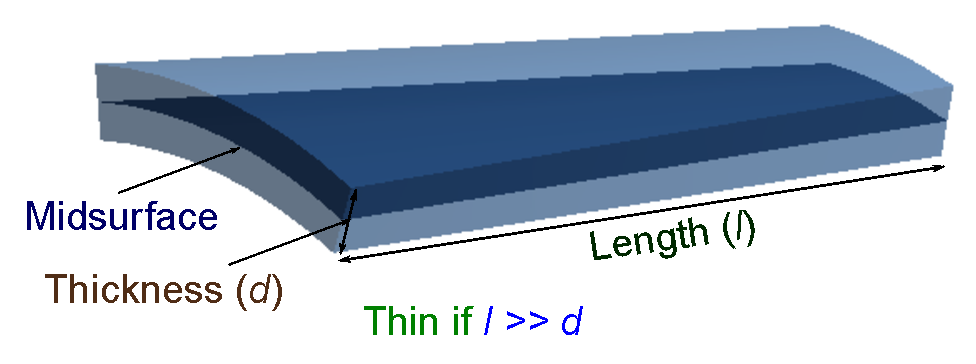
\includegraphics[scale=0.4]{../Common/images//Midsurf.pdf}
	\caption{Midsurface}
	\label{figure_Midsurf}
	\end{figure}

Most of the Midsurface extraction approaches are based on the final shape, represented typically by Boundary Representation (Brep) solid, do not use feature information. 

This paper demonstrate use of form features defined in terms of  Spatial Grammars notations in formulating Midsurface.
